\documentclass{article}

\usepackage[a4paper]{geometry}
\usepackage{lipsum}
\usepackage{graphicx}
\usepackage{amsmath}

\title{Project plan}
\author{Darcy Geyer, Sarah McCauley, Tin Nam Choi}
\date{2022\\October}

\begin{document}
  \maketitle{}
  
  \tableofcontents{}
  \setlength{\parindent}{0em}
  \setlength{\parskip}{1em}
  
  \pagebreak
  
  \section{Description}
  
  \subsection{The basics}
  The game is a text-based, turn-based, player-vs-CPU fighting and adventure game. Initially, the player chooses to catch 3 Pokemon from a given list of several Pokemon, each with unique details and stats (name, type, level, HP, basic attack, special attack, and defense). It is explained to the player that their objective is to reach a final landmark (the top of Mount Fuji), and that to get there, they will encounter enemies (CPUs), each holding 1 to 3 Pokemon. The player will have to battle and defeat 10 enemies, each being more difficult than the last. After defeating the 3rd, 6th, and 9th enemy, the player will encounter a new landmark, which will act as a checkpoint. If the player's pokemon are all defeated in a battle, the player will be returned to the most recently passed checkpoint, and if any enemies were defeated after passing the checkpoint, they will be reset, and the player will have to battle them again. The player wins the game once they have defeated all 10 enemies, and reached the top of Mount Fuji.
  
  \subsection{Pokemon}
  \begin{itemize}
    \item Name: Each Pokemon has a unique name. 
    \item Type: Each Pokemon possesses a type (either water, fire, or grass).
      \begin{itemize}
        \item Water is weak to grass attacks. 
        \item Fire is weak to water attacks. 
        \item Grass is weak to fire attacks. 
      \end{itemize}
    \item HP: Each Pokemon possesses a particular amount of health points (HP), when this reaches zero, the Pokemon is defeated. If a player's Pokemon is defeated in battle, the player is given a choice as to which of their remaining Pokemon they want to swap into the battle. If a CPU's Pokemon is defeated in battle, it is randomly swapped out with one of their remaining Pokemon. 
    \item Basic Attack: Each Pokemon has a basic attack. When this attack is used against an enemy Pokemon, a base-amount of HP is removed from it. If the attacking Pokemon's attack stat is higher than the opponent Pokemon's defense stat, additional HP is also removed from the opponent Pokemon. This additional amount is calculated using the difference in the attack stat of the attacking Pokemon and the defense stat of the opponent Pokemon. 
    \item Special Attack: Similar to the standard attack and functions the same. However, the special attack also possesses a 'type' (coinciding with that of the Pokemon). The type of special attack can be either water, fire, or grass. 
      \begin{itemize}
        \item Water special attacks:
          \begin{itemize}
            \item Take off $2\times$ (base amount + any difference in attack / defense) amount of HP against a fire-type Pokemon.
            \item Take off $\frac{1}{2}\times{}$ (base amount + any difference in attack / defense) amount of HP against a grass-type Pokemon.
            \item Take off the base amount + any difference in attack / defense amount of HP against another water-type Pokemon.
          \end{itemize}
        \item Fire special attacks:
          \begin{itemize}
            \item Take off $2\times$ (base amount + any difference in attack / defense) amount of HP against a grass-type Pokemon.
            \item Take off $\frac{1}{2}\times{}$ (base amount + any difference in attack / defense) amount of HP against a water-type Pokemon.
            \item Take off the base amount + any difference in attack / defense amount of HP against another fire-type Pokemon.
          \end{itemize}
        \item Grass special attacks:
          \begin{itemize}
            \item Take off $2\times$ (base amount + any difference in attack / defense) amount of HP against a water-type Pokemon.
            \item Take off $\frac{1}{2}\times{}$ (base amount + any difference in attack / defense) amount of HP against a fire-type Pokemon.
            \item Take off the base amount + any difference in attack / defense amount of HP against another grass-type Pokemon.
          \end{itemize}
      \end{itemize}
    \item Defense: If an attacking Pokemon's attack stat is higher than the opponent Pokemon's defense stat, additional HP is also removed from the opponent Pokemon. Otherwise, only a base amount of HP is removed from opponent Pokemon. A Pokemon can also use a 'defense move', which increases the defense stat of the Pokemon that used it for the duration of the battle. 
    \item Level: The level of each Pokemon is dependent on how much XP they have received. XP is gained by defeating other Pokemon. Defeating higher-level Pokemon gives the winning Pokemon more XP than lower-level Pokemon. After passing certain XP thresholds, a Pokemon can 'level up', which gives an increase to HP, attack, special attack, and defense. After passing certain level thresholds, a Pokemon can 'evolve', which gives a slightly larger increase to HP, basic attack, special attack, and defense, as well as altering the Pokemon's name and appearance. When a Pokemon evolves, it is also 'taught' a new move, which may be a basic or special attack, or a defense move. The new move will be stronger than previous moves of the same type.
  \end{itemize}
  
  \subsection{Battling}
  Battling is turn-based, meaning that the player and the CPU each take turns making a move. Before battling, the player will be given a choice as to which Pokemon they would like to send into battle first. For each turn, the player can either choose to use a basic attack, a special attack, a defensive move, or to swap Pokemon. Basic and special attacks, as well as defensive moves have been explained above. Choosing to swap Pokemon will give the player the opportunity to send a different Pokemon into battle. After each time the player makes a move, the CPU will be given the same options to make a move. It is explained above what occurs when a Pokemon reaches 0. If all of the player's Pokemon are defeated, the CPU will be determined the winner, and vice versa.
  
  \pagebreak

  \section{Potential classes}
  
  \subsection{Player}
  Data: 
  \begin{itemize}
    \item Pokemon owned
    \item Level 
  \end{itemize}
  Functions:
  \begin{itemize}
    \item Add/remove Pokemon owned
    \item Increment/decrement level
  \end{itemize}
  
  \subsubsection{Person}
  Data:
  \begin{itemize}
    \item Name
    \item Skill points (for leveling up)
  \end{itemize}
  Functions:
  \begin{itemize}
    \item Set name
    \item Increment/decrement skill points
    \item Get action from user
  \end{itemize}
  
  \subsubsection{Computer}
  Functions:
  \begin{itemize}
    \item Get action randomly
  \end{itemize}
    
  \subsection{Pokemon}
  Data:
  \begin{itemize}
    \item Name
    \item Type
    \item Level
    \item Health
    \item Attack
    \item Defense
    \item Speed
    \item Moves learnt
  \end{itemize}
  Functions:
  \begin{itemize}
    \item Increment/decrement level
    \item Increment/decrement health
    \item Increment/decrement attack
    \item Increment/decrement defense
    \item Increment/decrement speed
    \item Add/remove moves learnt
  \end{itemize}
  
  \subsection{Menu}
  Data:
  \begin{itemize}
    \item Title
    \item Options (vector)
  \end{itemize}
  Functions:
  \begin{itemize}
    \item Print menu
    \item Set title
    \item Set options
  \end{itemize}
  
  \pagebreak
  
  \section{Timeline}
  
  \subsection*{Mid-term break}
  \begin{itemize}
    \item Finalize plan
    \item Prototypical testing
  \end{itemize}
  
  \subsection*{Week 9}
  \begin{itemize}
    \item Submit plan
    \item Begin coding
  \end{itemize}
  
  \subsection*{Week 10}
  \begin{itemize}
    \item Finish version 1
  \end{itemize}
  
  \subsection*{Week 11}
  \begin{itemize}
    \item Finish coding
  \end{itemize}
  
  \pagebreak
  
  \section{User interface}
  
  The game will use a command-line interface. This will be done using the Menu class to display the options to the user, and the user will be able to select an option by typing the corresponding number. 
  
  \begin{center}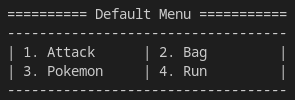
\includegraphics[height=2cm]{media/Menu.png}\end{center}
  
  \section{Unit testing and debugging}
    
\end{document}
